\documentclass[tikz]{standalone}
\usepackage{tikz}

\begin{document}

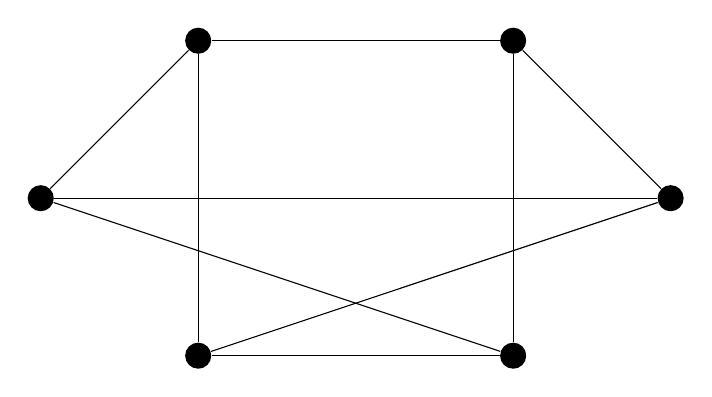
\begin{tikzpicture}[scale=2]
    % Define the vertices
    \node (A) at (-1, 0) [circle, fill=black] {};
    \node (B) at (1, 0) [circle, fill=black] {};
    \node (C) at (-2, -1) [circle, fill=black] {};
    \node (D) at (2, -1) [circle, fill=black] {};
    \node (E) at (-1, -2) [circle, fill=black] {};
    \node (F) at (1, -2) [circle, fill=black] {};

    % Draw the edges
    \draw (A) -- (B);
    \draw (A) -- (C);
    \draw (A) -- (E);
    \draw (B) -- (D);
    \draw (B) -- (F);
    \draw (C) -- (D);
    \draw (D) -- (E);
    \draw (E) -- (F);
    \draw (F) -- (C);

    % Add labels if needed
    % \node at (A) {A};
    % \node at (B) {B};
    % \node at (C) {C};
    % \node at (D) {D};
    % \node at (E) {E};
    % \node at (F) {F};

\end{tikzpicture}

\end{document}